\documentclass{jlreq}

\usepackage{titlesec}
\usepackage{listings}
\usepackage{fancyhdr}

\usepackage{url}

% \adjustbox
\usepackage{adjustbox}

% 数学
\usepackage{amssymb} 

% tcolorboxの設定
\usepackage[most]{tcolorbox} 
\tcbuselibrary{breakable}
\tcbuselibrary{skins}
\tcbuselibrary{listingsutf8}
% タイトルのフォーマットを変更
\titleformat{\title}
  {\centering\Huge\bfseries}
  {}
  {0em} 
  {}

\titleformat{\subtitle}
  {\centering\Large\itshape}
  {}
  {0em}
  {}

\titleformat{\subsubsection}[block]
  {\normalfont\normalsize\bfseries}
  {\arabic{subsubsection}.}
  {1em}
  {}

\titleformat{\section}[block]
  {\normalfont\large\bfseries}
  {\Roman{section}.}
  {1em} 
  {}
  [\titleline{\titlerule[1pt]}]

\titleformat{\subsection}[block]
  {\normalfont\normalsize\bfseries}
  {\roman{subsection}.}
  {1em}
  {}

% listingsの設定

\renewcommand{\lstlistingname}{コード}

\lstset{
	breaklines = true,
	language = Python,
	keywordstyle = {\bfseries \color[cmyk]{0,1,0,0}},
	commentstyle = {\itshape \color[cmyk]{1,0.4,1,0}},
	numbers = left,
	numberstyle = \tiny,
	stepnumber = 1,
	% frameとnumberの間の距離
	numbersep = 10pt,
	frame = single,
	basicstyle = \ttfamily,
	tabsize = 2,
	captionpos = t,
	backgroundcolor={\color[gray]{.90}},
	showstringspaces = false,
}

% headerの設定
\pagestyle{fancy}
\fancyhf{}

\fancyhead[RO,RE]{\rightmark}
\fancyhead[LO,LE]{\leftmark} 
\fancyfoot[C]{\thepage}

% tikzの設定
\usepackage{tikz}

% 定理環境
\newtcolorbox{theorembox}[1][]{
    enhanced,
    colback=white!95!green,
    colframe=green!40!black,
    coltitle=black,
    fonttitle=\bfseries,
    title=#1,
    attach boxed title to top left={yshift=-2mm, xshift=2mm},
    boxed title style={colback=green!30!white, size=small},
    drop fuzzy shadow,
    boxrule=0.5mm,
    sharp corners,
    top=4mm, bottom=4mm,
}

% 定義用のボックス環境
\newtcolorbox{definitionbox}[1][]{
    enhanced,
    title=#1, 
    attach boxed title to top left, 
    colback=white!95!blue,
    colbacktitle=white!10!blue!50!black,
    drop fuzzy shadow,
    boxrule=0.25mm,
}

% 問題用のボックス環境
\newtcolorbox{problem}[1][]{enhanced,
  colback=white!85!gray,
  drop fuzzy shadow,
  boxrule=0.3mm,
  arc=0mm,
  left=0pt,
  top=0pt,
  sharp corners,
  width=\textwidth,
  title=\textbf{問題},
  #1,
  breakable
}

\begin{document}
\section{線形代数と有名不等式}
\subsection{三角不等式}
\begin{theorembox}[三角不等式]
	$\boldsymbol{x}, \boldsymbol{y} \in \mathbb{R}^n$に対し、次の不等式が成り立つ。
	\begin{enumerate}
		\item  $\| \boldsymbol{x} \| - \| \boldsymbol{y} \| \leq \| \boldsymbol{x} + \boldsymbol{y} \| \leq \| \boldsymbol{x} \| + \| \boldsymbol{y} \|$
		\item $\| \boldsymbol{x} - \boldsymbol{y} \| \geq | \| \boldsymbol{x} \| - \| \boldsymbol{y} \| |$
	\end{enumerate}
\end{theorembox}

三角不等式を利用した問題を数問解いてみよう。

\begin{problem}
	次の2つの式を満たす平面ベクトル$\boldsymbol{x} = (x, y)$を考える。
	\begin{equation*}
		|\boldsymbol{x} + 2\boldsymbol{y}| = 1
	\end{equation*}	
	\begin{equation*}
		|2\boldsymbol{x} + \boldsymbol{y}| = 1
	\end{equation*}
	このとき、$|\boldsymbol{x} - 3 \boldsymbol{y}|$の最大値と最小値を求めよ。
\end{problem}

\begin{problem}
	関数$f(t) = \sqrt{t^2 + 1} + \sqrt{t^2 - 2t + 1}$ ($0 \leq t \leq 1$)が最小値をとる$t$の値を求めよ。
\end{problem}

\begin{problem}
	関数$g(t) = \sqrt{t^2 + 1}  \sqrt{t^2 - 2 t + 2}$ ($t > 1$)の最大値とそのときの$t$の値を求めよ。
\end{problem}

\subsection{コーシー・シュワルツの不等式}

\begin{theorembox}[コーシー・シュワルツの不等式]
	$\boldsymbol{x}, \boldsymbol{y} \in \mathbb{R}^n$に対し、次の不等式が成り立つ。
	\begin{equation*}
		| \boldsymbol{x} \cdot \boldsymbol{y} | \leq \| \boldsymbol{x} \| \| \boldsymbol{y} \|
	\end{equation*}
\end{theorembox}

コーシー・シュワルツの不等式を利用した問題を数問解いてみよう。

\begin{problem}
	$x, y, z > 0$, $x + y + z = 1$のとき、以下に答えよ。
	\begin{enumerate}
		\item $x^2 + y^2 + z^2$の最小値
		\item $\frac{1}{x} + \frac{1}{y} + \frac{1}{z}$の最小値
	\end{enumerate}
\end{problem}

参考
\begin{itemize}
  \item \url{https://www.chart.co.jp/subject/sugaku/suken_tsushin/76/76-3.pdf}
  \item \url{https://mathematicsgarden.com/cschwarzprac/}
\end{itemize}

\section{座標空間と数ベクトル空間}
ここでは2次元と3次元の座標空間の問題を解いてみよう。

\begin{theorembox}[直線のパラメータ表示]
  直線$l$上の1点$\boldsymbol{p} = (x_0, y_0, z_0)$と方向ベクトル$\boldsymbol{a} = (a, b, c)$が与えられたとき、直線$l$上の任意の点$\boldsymbol{r} = (x, y, z)$は次のように表される。

  \begin{equation*}
    \begin{pmatrix}
      x \\ y \\ z 
    \end{pmatrix}
    = \boldsymbol{p} + t \boldsymbol{a} = 
    \begin{pmatrix}
      x_0 + t a \\ y_0 + t b \\ z_0 + t c
    \end{pmatrix}
  \end{equation*}
  パラメータ$t$を消去すると、直線$l$の方程式は次のように表される。

  \begin{equation*}
    \frac{x - x_0}{a} = \frac{y - y_0}{b} = \frac{z - z_0}{c}
  \end{equation*}
\end{theorembox}

\begin{theorembox}[平面の方程式]
  平面上の点$\boldsymbol{p} = (x_0, y_0, z_0)$と法線ベクトル$\boldsymbol{n} = (a, b, c)$が与えられたとき、平面上の任意の点$\boldsymbol{r} = (x, y, z)$は
  $\boldsymbol{n} \cdot (\boldsymbol{r} - \boldsymbol{p}) = 0$を満たす。よって
  \begin{equation*}
    a(x - x_0) + b(y - y_0) + c(z - z_0) = 0
  \end{equation*}

  となる。これを整理すると、
  \begin{equation*}
    ax + by + cz = a x_0 + b y_0 + c z_0 = d
  \end{equation*}
   となり、これが平面の方程式となる。
\end{theorembox}

それでは問題を解いてみよう。

\begin{problem}
  点$(0, 2, 1)$を通り、$\boldsymbol{n} = (1, -2, 3)$を法線ベクトルとする平面の方程式を求めよ。
\end{problem}

\begin{problem}
  $xyz$平面の平面$P: 2x - y + 3z = 1$に関して、点$A \begin{pmatrix} 1 \\ 2 \\ 4 \end{pmatrix}$と対照な
  点$A'$を求めよ。

  \dotfill
  解答 \\
\end{problem}

\section{行列式}
行列式は大学院入試数学において基本中の基本の問題である。行列式に関する問題を解いて理解を深めよう。
\begin{problem}
  以下の行列の行列式を求めよ。
  \begin{center}
    \begin{tabular}{cc}
      $\displaystyle
        \begin{pmatrix}
          2015 & 2014 & 2014 \\
          2015 & 2015 & 2014 \\
          2015 & 2015 & 2015
        \end{pmatrix}
      $
      & \hspace{2cm} % スペースを空けるための調整
      $\displaystyle
        \begin{pmatrix}
          1 & 3 & 2 & -1 \\
          2 & 0 & 1 & -2 \\
          -1 & 5 & 1 & 1 \\
          2 & 7 & -6 & 3
        \end{pmatrix}
      $
    \end{tabular}
  \end{center}
  \dotfill

  解答 \\
  (1) \\
  行列式は\textbf{余因子展開}により行または列で展開することができる。また、行列式は基本変形に関して以下の性質があります。

  \begin{itemize}
    \item 行列の行(列)を交換すると、行列式の符号が変わる。
    \item 行列の行(列)に定数をかけると、行列式もその定数倍になる。
    \item 行列の行(列)に他の行(列)の定数倍を加えると、行列式は変わらない。
  \end{itemize}

  これらの性質を用いて計算します。

  \begin{equation*}
    \det \begin{pmatrix}
      2015 & 2014 & 2014 \\
      2015 & 2015 & 2014 \\
      2015 & 2015 & 2015
    \end{pmatrix} = \det \begin{pmatrix}
      2015 & 2014 & 2014 \\
      0 & 1 & 0 \\
      0 & 1 & 1
    \end{pmatrix} = 2015 \det \begin{pmatrix}
      1 & 0 \\
      1 & 1
    \end{pmatrix} = 2015
  \end{equation*}

  (2) \\
  行基本変形と余因子展開を用いて計算する。
  
  \begin{equation*}
    \det \begin{pmatrix}
      1 & 3 & 2 & -1 \\
      2 & 0 & 1 & -2 \\
      -1 & 5 & 1 & 1 \\
      2 & 7 & -6 & 3
    \end{pmatrix} = \det \begin{pmatrix}
      1 & 3 & 2 & -1 \\
      0 & -6 & -3 & 0 \\
      0 & 8 & 3 & 0 \\
      0 & 1 & -10 & 5
    \end{pmatrix}
  \end{equation*}
  \begin{equation*}
    = \det \begin{pmatrix}
      -6 & -3 & 0 \\
      8 & 3 & 0 \\
      1 & -10 & 5
    \end{pmatrix} = (-1) ^ {3 + 3} \times 5 \times \det \begin{pmatrix}
      -6 & -3 \\
      8 & 3
    \end{pmatrix} = 5 \times 6 = 30
  \end{equation*}
\end{problem}

\begin{tcolorbox}[enhanced, title=コラム1 行列式の幾何的性質, breakable, colback=white, drop fuzzy shadow, attach boxed title to top center={yshift*=0.1cm}]
  行列式を2次元平面で考えると、行列式は2つのベクトルが張る平行四辺形の面積を表す。平行四辺形の面積をとすると、
  \begin{equation*}
    \det \begin{pmatrix}
      a & b \\
      c & d
    \end{pmatrix} = ad - bc
  \end{equation*}
  が成り立つ。証明は平行四辺形を囲う長方形から三角形を切り出すことで導出できる。行列$A = \begin{pmatrix}a & c \\ b & d\end{pmatrix}$
  は単位ベクトルからなる正方形を変換する行列と考えることができる。つまり、行列式は正方形の面積の拡大率を表すとみなせる。また、
  $\det A = 0$、つまり拡大率が0になるときは、2つのベクトルが一直線上にあることを意味する。2次元で考えたが、3次元以上でも同様の性質が成り立つ。

  「行列 平行四辺形」と調べると面白い関係を述べた記事が見つかる。
  \vspace{0.5cm}
  \begin{center}
    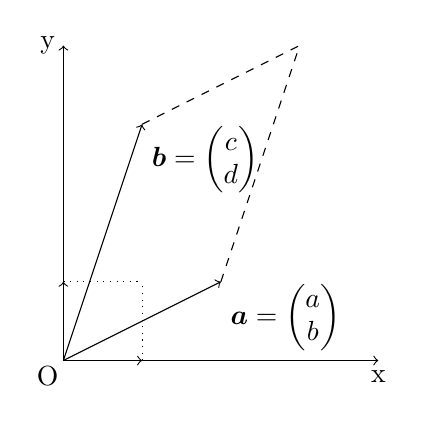
\begin{tikzpicture}
        \draw [->] (0, 0) -- (4, 0);
        \draw [->] (0, 0) -- (0, 4);

        % ベクトルを描画
        \draw [->] (0, 0) -- (2, 1);
        \draw [->] (0, 0) -- (1, 3);

        % 並行4辺形を描画
        \draw [dashed] (2, 1) -- (3, 4);
        \draw [dashed] (1, 3) -- (3, 4);

        % ベクトルを表示
        \node at (2, 0) [anchor = south west] {$\boldsymbol{a} = \begin{pmatrix} a \\ b \end{pmatrix}$};
        \node at (1, 2) [anchor = south west] {$\boldsymbol{b} = \begin{pmatrix} c \\ d \end{pmatrix}$};

        % 単位ベクトルからなる正方形
        \draw [->] (0, 0) -- (1, 0);
        \draw [->] (0, 0) -- (0, 1);
        \draw [dotted] (1, 0) -- (1, 1);
        \draw [dotted] (0, 1) -- (1, 1);
    
        % 文字を描画
        \node at (-0.2, -0.2) {O};
        \node at (4, -0.2) {x};
        \node at (-0.2, 4) {y};
    \end{tikzpicture}
    \end{center}
\end{tcolorbox}

次に行列式の累乗の問題を扱う。

\begin{problem}
  Aを$n$次正方行列、$I$を単位行列とするとき、以下の問に答えよ。

  \begin{equation*}
    A = \begin{pmatrix}
      I - A & A \\
      -A & I + A
    \end{pmatrix}
  \end{equation*}
  (1) \\
  $A^3$を求めよ。
  (2) \\
  $A^m$を求めよ。

  \dotfill

  解答 \\
  行列の累乗を求める問題には行列の対角化やケーリーハミルトンの定理を用いることがある。今回は行列の性質を用いて解く。
  行列の対角化は具体的に行列の成分がわかっていない時には難しいため、行列の性質を用いて解く。
  (1) \\
  $A^3$を求めるためには、$A^2$を求める必要がある。$I$が単位行列であることに注意すると、

  \begin{equation*}
    A^2 = \begin{pmatrix}
      I - 2A & 2A \\
      -2A & I + 2A
    \end{pmatrix}
  \end{equation*}
  より、$A^3$を計算すると以下の様になる。
  \begin{equation*}
    A^3 = \begin{pmatrix}
      I - 3A & 3A \\
      -3 A & I + 3A
    \end{pmatrix}
  \end{equation*}

  (2) \\
  $A^m$は以下の様に現させることが予想される。
  \begin{equation*}
    A^m = \begin{pmatrix}
      I - mA & mA \\
      -mA & I + mA
    \end{pmatrix}
  \end{equation*}
  これを数学的帰納法を用いて証明する。

  $m = 1, 2, 3$は(1)より成り立つ。$m \geq 4$のとき、$A^{m - 1}$を仮定すると、
  \begin{equation*}
    A^{m} = A^{m - 1} A = \begin{pmatrix}
      I - (m - 1)A & (m - 1)A \\
      -(m - 1)A & I + (m - 1)A
    \end{pmatrix} \begin{pmatrix}
      I - A & A \\
      -A & I + A
    \end{pmatrix}
    = \begin{pmatrix}
      I - mA & mA \\
      -mA & I + mA
    \end{pmatrix}
  \end{equation*} 
\end{problem}

与えられた条件から成分の分布を求める行列方程式の典型問題を扱う。

\begin{problem}
  3次の正方行列に対して次の問題に答えよ。

  \begin{equation*}
    A = \begin{pmatrix}
      1 & 0 & 0 \\
      0 & 2 & 0 \\
      0 & 0 & 3
    \end{pmatrix}, \hspace{1cm}
    B = \begin{pmatrix}
      1 & 0 & 0 \\
      0 & 2 & 0 \\
      0 & 0 & 1
    \end{pmatrix}, \hspace{1cm}
    C = \begin{pmatrix}
      1 & 0 & 1 \\
      0 & 2 & 0 \\
      -1 & 0 & 1
    \end{pmatrix}
  \end{equation*}
  (1) $AX = XA$を満たす行列$X$は対角行列であることを示せ。 \\
  (2) $BX = XB, BY = YB, XY = YX$を満たす行列$X, Y$の例を挙げよ。 \\
  (3) $AX = XA, CX = XC$を満たす行列$X$は$a I + b B$と表せることを示せ。 

  \dotfill

  解答 \\
  (1) \\
  行列$A, X$の片方が対角行列という簡単な形式になっているので、
  \begin{equation*}
    X = \begin{pmatrix}
      x_{11} & x_{12} & x_{13} \\
      x_{21} & x_{22} & x_{23} \\
      x_{31} & x_{32} & x_{33}
    \end{pmatrix}
  \end{equation*}
  と行列$X$を一般的な形で表すして証明しよう。
\end{problem}

\section{連立方程式と階数}
\begin{definitionbox}[階数]
  任意の行列$A$は行基本変形を繰り返すことによって、\textbf{階段行列}にすることができる。このとき、この階段行列
  のなかの少なくとも1つは0ではない成分を持つ行の個数$r$を行列$A$の\textbf{階数}といい、$\text{rank} A$で表す。

  任意の行基本変形に対して、行列$A$の階数は一意に定まる。
\end{definitionbox}

連立方程式の解と階数に関する定理を紹介する。

\begin{theorembox}[連立方程式と階数]
  $n$元連立一次方程式に関して、$\boldsymbol{A}$を係数行列、$\boldsymbol{b}$を定数ベクトルとして$\boldsymbol{A} \boldsymbol{b}$が拡大係数行列とする。
  このとき、次のことが成り立つ。
  
  \begin{itemize}
    \item rank $\boldsymbol{A} = $ rank $\boldsymbol{A} \boldsymbol{b} = r$のとき、連立方程式は解を持つ。
    \item $n > \text{rank} A$なら、連立方程式は無数の解を持つ。
    \item $n = $\text{rank} $\boldsymbol{A} = $ rank $\boldsymbol{A} \boldsymbol{b} = r$のとき、連立方程式はただ1つの解を持つ。
    \item rank $\boldsymbol{A} = $ rank $\boldsymbol{A} \boldsymbol{b} = r < n$のとき、連立方程式は解を持たない。
  \end{itemize}
\end{theorembox}

一元連立方程式の問題を解いてみよう。

\begin{problem}
  以下の連立一次方程式を解け。
  \begin{equation*}
    (1)  \left\{ \,
    \begin{aligned}
      5x_1 + 2x_2 + 3 x_3 = 28 \\
      x_1 + 3 x_2 + x_3 = 15 \\
      2x_1 + 2x_2 + 2 x_3 = 18
    \end{aligned}
\right.
  \end{equation*}

  \begin{equation*}
    (2) \left\{ \,
    \begin{aligned}
      x_1 - x_2 + 2 x_3 = 0 \\
      -2x_1 - x_2 - 2 x_3 = 0 \\
      4x_1 - 7x_2 + 10 x_3 = 0
    \end{aligned}
\right.
  \end{equation*}

  \begin{equation*}
    (3) \left\{ \,
    \begin{aligned}
      x_1 + x_2 + x_3 = 3 \\
      3 x_1 + 2 x_2 - 2 x_3 = 5 \\
      6 x_1 + 5 x_2 + x_3 = 14
    \end{aligned}
\right.
  \end{equation*}
  \dotfill

  解答 \\
  (1) \\
  連立一次方程式の係数行列と拡大係数行列をそれぞれ$A, [A|b]$とすると、
  \begin{equation*}
    [A|b] = \begin{pmatrix}
      5 & 2 & 3 & 28 \\
      1 & 3 & 1 & 15 \\
      2 & 2 & 2 & 18
    \end{pmatrix} \to \begin{pmatrix}
      1 & 0 & 0 & 2 \\
      0 & 1 & 0 & 3 \\
      0 & 0 & 1 & 4
    \end{pmatrix}
  \end{equation*}
  のようになるので、一元連立方程式の解は$x_1 = 2, x_2 = 3, x_3 = 4$である。

  (2) \\

  (3) \\
\end{problem}

次に、行列の世界の積の逆元を意味する\textbf{逆行列}について紹介する。

\begin{definitionbox}[逆行列]
  正方行列$A$に対して、$A$と積をとると単位行列$I$が得られるとき、$A$の逆行列$A^{-1}$が存在するといい、
  $A A^{-1} = A^{-1} A = I$を満たす。 逆行列が存在するとき、$A$は\textbf{正則行列}であるという。
\end{definitionbox}

\begin{theorembox}[逆行列と余因子行列]
  $n$次正方行列$A$が正則であるとき、その逆行列$A^{-1}$は次のように表される。
  
  \begin{equation*}
    A^{-1} = \frac{1}{\det A} \tilde{A}
  \end{equation*}

  $\tilde{A}$は$A$の余因子行列であり、$A$の余因子$C_{ij}$は次のように表される。
  \begin{equation*}
    C_{ij} = \tilde{A_{ji}}
  \end{equation*}
  ここで、$\tilde{A_{ji}}$は$A$の$i$行$j$列を取り除いた行列の行列式に$(-1)^{i+j}$をかけたものである。
\end{theorembox}

逆行列に関する問題を解いてみよう。\textbf{掃き出し法}によって逆行列を求める問題を解いてみよう。

\begin{problem}
  \begin{equation*}
    A = \begin{pmatrix}
      2 & 1 & 1 \\
      1 & 1 & 1 \\
      -2 & 0 & 1
    \end{pmatrix}
  \end{equation*}
  \dotfill

  解答 \\
  掃き出し法とは、$A \boldsymbol{X} = \boldsymbol{I}$の形になるように、
  \begin{equation*}
    \begin{pmatrix}
      A & I
    \end{pmatrix} \to \begin{pmatrix}
      I & A^{-1}
    \end{pmatrix}
  \end{equation*}
  ように、行列$A$を$I$に変換する方法である。この方法を用いて、
  \begin{equation*}
    \begin{pmatrix}
      2 & 1 & 1 & 1 & 0 & 0 \\
      1 & 1 & 1 & 0 & 1 & 0 \\
      -2 & 0 & 1 & 0 & 0 & 1
    \end{pmatrix} \to \begin{pmatrix}
      1 & 0 & 0 & 1 & -1 & 0 \\
      0 & 1 & 0 & -3 & 4 & -1 \\
      0 & 0 & 1 & 2 & -2 & 1
    \end{pmatrix}
  \end{equation*}
\end{problem}

\section{線形写像}

\subsection{線形写像}
\begin{definitionbox}[線形写像]
  $\forall \boldsymbol{x}, \boldsymbol{y} \in \mathbb{R}^n$, $\forall \lambda \in \mathbb{R}$に対して、次の2つの条件を満たす写像$f: \mathbb{R}^n \to \mathbb{R}^m$を\textbf{線形写像}という。

  \begin{enumerate}
    \item $f(\boldsymbol{x} + \boldsymbol{y}) = f(\boldsymbol{x}) + f(\boldsymbol{y})$
    \item $f(\lambda \boldsymbol{x}) = \lambda f(\boldsymbol{x})$
  \end{enumerate}
\end{definitionbox}

\subsection{表現行列}

\begin{theorembox}[表現行列]
  どんな線形写像$f: \mathbb{R}^n \to \mathbb{R}^m$に対しても、ある一意な行列$A$が存在して、
  \begin{equation*}
    f(\boldsymbol{x}) = A \boldsymbol{x}
  \end{equation*}
  と表される。この行列$A$を$f$の\textbf{表現行列}という。
\end{theorembox}

表現行列に関わる問題を解いてみよう。

\begin{problem}
  線形写像$f: \mathbb{R}^2 \to \mathbb{R}^2$が次のように定義されるとき、$f$の表現行列を求めよ。
  \begin{equation*}
    \text{fは}y = (\tan x) \text{での鏡映}
  \end{equation*}
  \dotfill

  解答 \\
  線形写像の表現行列を求めるには、以下の2つの方法がある。
  \begin{itemize}
    \item 定義域の写像の元を一般的に表して、終域の元を求める。
    \item 基底を用いて表現行列を求める。
  \end{itemize}

  今回は2の方法を用いて表現行列を求める。$xy$座標では$(1, 0)$と$(0, 1)$を基底として用いることができるので、
  それぞれの写像$f$による像を求める。

  \begin{equation*}
    f(1, 0) = (\tan 1, 0) = (\cos 2 x, \sin 2 x)
  \end{equation*}
  \begin{equation*}
    f(0, 1) = (0, \tan 1) = (\sin 2 x, -\cos 2 x)
  \end{equation*}
  よって求める表現行列は、
  \begin{equation*}
    A = \begin{pmatrix}
      \cos 2 x & \sin 2 x \\
      \sin 2 x & -\cos 2 x
    \end{pmatrix}
  \end{equation*}
\end{problem}

\begin{problem}
  $\mathbb{R}^3$の点$A$を、$A$から平面$x - 2y + z = 0$へ下ろした垂線の足に写す線形写像の表現行列を求めよ。
  \dotfill

  解答 \\
  $\mathbb{R}^3$の単位ベクトルがどのように写るかを考える。$\boldsymbol{e}_1 = (1, 0, 0)$に対して
  法線ベクトル$\boldsymbol{n} = (1, -2, 1)$を用いて、$\boldsymbol{e}_1$から平面へ下ろした垂線の足は
  \begin{equation*}
    \boldsymbol{n} + t \boldsymbol{e}_1 = (1 + t, -2t, t)
  \end{equation*}
  これが平面$x - 2y + z = 0$上にあればよいので、$t = -\frac{1}{6}$となる。どうの様にすることで、
  $\boldsymbol{e}_2 = (0, 1, 0)$と$\boldsymbol{e}_3 = (0, 0, 1)$が写るかを考えると、求める表現行列は

  \begin{equation*}
    A = \begin{pmatrix}
      \frac{5}{6} & \frac{1}{3} & -\frac{1}{6} \\
      -\frac{1}{3} & \frac{1}{3} & \frac{1}{3} \\
      -\frac{1}{6} & \frac{1}{3} & \frac{5}{6}
    \end{pmatrix}
  \end{equation*}
\end{problem}

\section{部分空間}
\begin{definitionbox}[部分空間]
  ベクトル空間$V$の部分集合$W$が次の2つの条件を満たすとき、$W$は$V$の\textbf{部分空間}であるという。

  \begin{enumerate}
    \item $\boldsymbol{0} \in W$
    \item $\boldsymbol{u}, \boldsymbol{v} \in W$に対して、$\boldsymbol{u} + \boldsymbol{v} \in W$
    \item $\lambda \boldsymbol{u} \in W$
  \end{enumerate}
\end{definitionbox}

部分空間を扱った問題を解いてみよう。

\begin{problem}
  次の$W$が$\mathbb{R}^3$の部分空間となるか判定せよ。
  \begin{equation*}
    W = \{ (x, y, z) \in \mathbb{R}^3 | 3x - z = y + 2z = x - y \}
  \end{equation*}

  \dotfill

  解答 \\
  まず、$\boldsymbol{0} = (0, 0, 0) \in W$である。
\end{problem}

\section{基底と次元}
\begin{definitionbox}[基底]
  ベクトル空間$V$のベクトルたち$\boldsymbol{v}_1, \boldsymbol{v}_2, \ldots, \boldsymbol{v}_n$が次の2つの条件を満たすとき、これらは$V$の\textbf{基底}をなすという。

  \begin{enumerate}
    \item $\boldsymbol{v}_1, \boldsymbol{v}_2, \ldots, \boldsymbol{v}_n$は$V$の1次独立である。
    \item $V$の任意のベクトル$\boldsymbol{v}$は$\boldsymbol{v}_1, \boldsymbol{v}_2, \ldots, \boldsymbol{v}_n$の線形結合で表される。
  \end{enumerate}
\end{definitionbox}

\begin{definitionbox}[次元]
  ベクトル空間$V$の基底の数を$V$の\textbf{次元}といい、$\dim V$で表す。
  $V$が有限個のベクトルで生成できないとき、$V$は無限次元であるという($\dim V = \infty$)。
\end{definitionbox}

\begin{definitionbox}[一次独立と一次従属]
  ベクトル$\boldsymbol{v}_1, \boldsymbol{v}_2, \ldots, \boldsymbol{v}_n$が\textbf{一次独立}であるとは、
  $\lambda_1, \lambda_2, \cdots, \lambda_n \in \mathbb{R}$に対して、
  \begin{equation*}
    \lambda_1 \boldsymbol{v}_1 + \lambda_2 \boldsymbol{v}_2 + \cdots + \lambda_n \boldsymbol{v}_n = \boldsymbol{0}
  \end{equation*}
  が成り立つとき、$\lambda_1 = \lambda_2 = \cdots = \lambda_n = 0$に限るをいう。

  それ以外のとき、$\boldsymbol{v}_1, \boldsymbol{v}_2, \ldots, \boldsymbol{v}_n$は\textbf{一次従属}であるという。
\end{definitionbox}

一次独立について重要な定理を紹介する。

\begin{theorembox}[一次独立と同値な条件]
  ベクトル$\boldsymbol{v}_1, \boldsymbol{v}_2, \ldots, \boldsymbol{v}_n$が一次独立であるための必要十分条件は、以下のいずれかが成り立つことである。
  $V= \mathbb{R}^n$のとき、

  \begin{itemize}
    \item $\boldsymbol{v}_1, \boldsymbol{v}_2, \ldots, \boldsymbol{v}_n \in \mathbb{R}^n$に対し、$n \times k$行列$A = (\boldsymbol{v}_1, \boldsymbol{v}_2, \ldots, \boldsymbol{v}_n)$のランクが$k$である。
    \item $\det A \neq 0$
    \item $A$が正則行列である。
    \item $<\boldsymbol{v}_1, \boldsymbol{v}_2, \ldots, \boldsymbol{v}_n> = \mathbb{R}^n$
  \end{itemize}
\end{theorembox}
\begin{problem}
  次のベクトルの組みが一次独立であるか判定せよ。
  \begin{equation*}
    \boldsymbol{a}_1 = \begin{pmatrix} 2 \\ 3 \\ -1  \\ 1 \end{pmatrix}, \boldsymbol{a}_2 = \begin{pmatrix} -3 \\ 2 \\ 0 \\ -2 \end{pmatrix}, \boldsymbol{a}_3 = \begin{pmatrix} 1 \\ -5 \\ -1 \\ 1 \end{pmatrix}
  \end{equation*}

  \dotfill

  解答 \\
  行列
  \begin{equation*}
    A = \begin{pmatrix}
      2 & -3 & 1 \\
      3 & 2 & -5 \\
      -1 & 0 & -1 \\
      1 & -2 & 1
    \end{pmatrix}
  \end{equation*}
  に対して行基本変形をして簡約化して階段行列を求めると、
  \begin{equation*}
    \begin{pmatrix}
      1 & 0 & 1 \\
      0 & 1 & 0 \\
      0 & 0 & 1 \\
      0 & 0 & 0
    \end{pmatrix}
  \end{equation*}
  となるので、$rank A = 3$であり、$\boldsymbol{a}_1, \boldsymbol{a}_2, \boldsymbol{a}_3$は一次独立である。
\end{problem}


\begin{definitionbox}[基底の変換行列]
  $V$を$\mathbb{R}$上のベクトル空間とし、$\dim V = n$とする。$V$の2つの基底
  \begin{equation*}
   A:  \boldsymbol{u}_1, \boldsymbol{u}_2, \ldots, \boldsymbol{u}_n
  \end{equation*}
  \begin{equation*}
    B: \boldsymbol{v}_1, \boldsymbol{v}_2, \ldots, \boldsymbol{v}_n
  \end{equation*}
  が与えられたとき、これらの基底の間の変換行列$P$は次のように定義される。

  \begin{equation*}
    \begin{pmatrix}
      \boldsymbol{v}_1 & \boldsymbol{v}_2 & \cdots & \boldsymbol{v}_n
    \end{pmatrix} = 
    \begin{pmatrix}
      \boldsymbol{u}_1 & \boldsymbol{u}_2 & \cdots & \boldsymbol{u}_n
    \end{pmatrix}
    \begin{pmatrix}
      p_{11} & p_{12} & \cdots & p_{1n} \\
      p_{21} & p_{22} & \cdots & p_{2n} \\
      \vdots & \vdots & \ddots & \vdots \\
      p_{n1} & p_{n2} & \cdots & p_{nn}
    \end{pmatrix}
  \end{equation*}
  行列$P$を$A$から$B$への基底の変換行列という。
\end{definitionbox}

\begin{problem}
  \begin{equation*}
    \boldsymbol{a}_1 = \begin{pmatrix}
      2 \\ 0 \\ 1
    \end{pmatrix}, \boldsymbol{a}_2 = \begin{pmatrix}
      1 \\ 1 \\ 0
    \end{pmatrix}, \boldsymbol{a}_3 = \begin{pmatrix}
      0 \\ -1 \\ 1
    \end{pmatrix}
  \end{equation*}
  
  \begin{equation*}
    \boldsymbol{b}_1 = \begin{pmatrix}
      1 \\ -1 \\ 2
    \end{pmatrix}, \boldsymbol{b}_2 = \begin{pmatrix}
      2 \\ 2 \\ -1
    \end{pmatrix}, \boldsymbol{b}_3 = \begin{pmatrix}
      0 \\ 1 \\ -1
    \end{pmatrix}
  \end{equation*}
  として、$\mathbb{R}^3$ 
  の基底$A = \{ \boldsymbol{a}_1, \boldsymbol{a}_2, \boldsymbol{a}_3 \}$から$\mathbb{R}^3$の基底$B = \{ \boldsymbol{b}_1, \boldsymbol{b}_2, \boldsymbol{b}_3 \}$への変換行列$P$を求めよ。

  \dotfill

  解答 \\
  定義より、$(\boldsymbol{b}_1, \boldsymbol{b}_2, \boldsymbol{b}_3) = ( \boldsymbol{a}_1, \boldsymbol{a}_2, \boldsymbol{a}_3) P$であるので、
  $A = (\boldsymbol{a}_1, \boldsymbol{a}_2, \boldsymbol{a}_3)$, $B = (\boldsymbol{b}_1, \boldsymbol{b}_2, \boldsymbol{b}_3)$として、
  $P = A^{-1} B$を求める。
  \begin{equation*}
    A^{-1} = \begin{pmatrix}
      1 & -1 & -1 \\
      -1 & 2 & 2 \\
      -1 & 1 & 2
    \end{pmatrix}
  \end{equation*}
  となるので、
  \begin{equation*}
    P = A^{-1} B = \begin{pmatrix}
      0 & 1 & 0 \\
      1 & 0 & 0 \\
      2 & -2 & -1
    \end{pmatrix}
  \end{equation*}

  別解 \\
  掃き出し法を用いて直接$P = A^{-1} B$を求めることもできる。($(A B)$の形になるように行列を並べて、$A$の部分を単位行列に変換する)

  \begin{equation*}
    \begin{pmatrix}
      2 & 1 & 0 & 1 & 2 & 0 \\
      0 & 1 & -1 & -1 & 2 & 1 \\
      1 & 0 & 1 & 0 & -1 & -1
    \end{pmatrix} \to \begin{pmatrix}
      1 & 0 & 0 & 0 & 1 & 0 \\
      0 & 1 & 0 & 0 & 1 & 1 \\
      0 & 0 & 1 & 0 & -1 & -1
    \end{pmatrix}
  \end{equation*}
\end{problem}

参考
\begin{itemize}
  \item \url{https://uxhpu.net/mathematics/change_of_basis/}
\end{itemize}

\end{document}